\documentclass[
	style=aggie,
	mode=present,
	size=10pt,
	paper=screen,
	orient=landscape,
	display=slides,
]{powerdot}

\usepackage{psfrag,graphicx,epsfig,array,subfigure}
\usepackage{amsmath,amsfonts,amssymb,amsthm,amsxtra}
\usepackage{bm}
\usepackage{hyperref}
\usepackage{multirow,booktabs}

\newcommand{\norm}[1]	{\lVert#1\rVert}
\newcommand{\NTF}		{\mathop\text{NTF}}
\newcommand{\STF}		{\mathop\text{STF}}
\newcommand{\DS}		{$\Delta\Sigma$\space}
\newcommand{\twosub}[2]{\begin{subarray}{l}{#1}\\{#2}\end{subarray}}

\makeatletter
\newcommand*\dashline{\rotatebox[origin=c]{90}{$\dabar@\dabar@\dabar@$}}
\makeatother

\pdsetup{
  lf=MSEE Oral Defense,
  rf=Matthew E. Jackson,
  logohook=c,
  logopos={.5\slidewidth,.038\slideheight},
  logocmd={
\includegraphics[scale=.3]{redlogo}}
%   logopos={.5\slidewidth,.027\slideheight},
%   logocmd={
\includegraphics[scale=.24]{redlogo}},
%   palette=Sea
}

\title{Optimal Design of Discrete-Time \DS Modulators}
\author{
\textbf{Matthew E. Jackson}\\
\\
\begin{footnotesize}Advisor: Peter A. Stubberud, Ph.D.\end{footnotesize}\\
\\
\begin{scriptsize}University of Nevada - Las Vegas\end{scriptsize}\\
\begin{scriptsize}\textit{Department of Electrical and Computer
Engineering}\end{scriptsize}\\
\begin{scriptsize}4505 Maryland Parkway\end{scriptsize}\\
\begin{scriptsize}Las Vegas, Nevada, USA\end{scriptsize}\\
}
\date{}

\begin{document}

\maketitle

%%%%%%%%%%%%%%%%%%%%%%%%%%%%%%%%%%%%%%%%
%% OVERVIEW SLIDE
\begin{slide}[toc=,bm=]{Overview}
	\begin{itemize}[type=1]
		\item Introduction
  		\begin{itemize}
  			\item Motivation: Optimal Design of \DS Modulators
   			\item Rationale: Global Optimization of Multimodal Performance Surfaces 
				  which Characterize Optimal IIR Filters 
  			\item Genetic Algorithms: Structure and Operational Theory \pause
		\end{itemize}
  		\item Hybrid Orthogonal Genetic (HOG) Algorithm
  		\begin{itemize}
   			\item Operational Theory and Implementation
   			\item \textit{Taguchi Method} and \textit{Design of Experiments}
 			\item Global Optimizer Application Examples \pause
  		\end{itemize}
  		\item Optimal Discrete-Time \DS Modulator Design and Results
  		\begin{itemize}
   			\item HOG Algorithm Implementation
   			\item \DS Modulator Modeling, Simulation, and Analysis
   			\item Results \pause
  		\end{itemize}
  		\item Conclusion
	\end{itemize}
\end{slide}
%%%%%%%%%%%%%%%%%%%%%%%%%%%%%%%%

%%%%%%%%%%%%%%%%%%%%%%%%%%%%%%%%%%%%%%%%%%%%%%%%%%%%%%%%%%%%%%%%%%%%%%%%%%%%%%%%
%% BACKGROUND
%%%%%%%%%%%%%%%%%%%%%%%%%%%%%%%%%%%%%%%%%%%%%%%%%%%%%%%%%%%%%%%%%%%%%%%%%%%%%%%%
\section[slide=true]{Introduction}

%%%%%%%%%%%%%%%%%%%%%%%%%%%%%%%%
%%% MOTIVATION 
\begin{slide}{Motivation}
\onslide*{1}{
	\begin{large}
	Optimal Design of $\Delta\Sigma$ Modulator Data Converters 
	\end{large}
	%---------------------------------------------------------------------------------
	\begin{figure}[h!]
	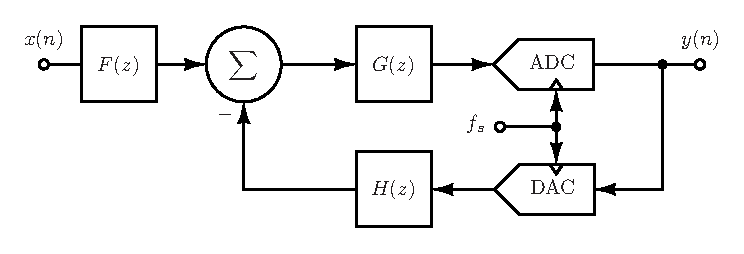
\includegraphics[width=0.8\textwidth]{DTDSM}
	\end{figure}	
	%---------------------------------------------------------------------------------
	\begin{itemize}
		\item Simple analog circuitry and low order quantizer simplifies hardware
		requirements
		\vspace{2mm}
		\item Utilizes oversampling and noise-shaping to achieve high
		Signal-to-Noise Ratio (SNR) and improved Dynamic Range
		(DR)
	\end{itemize}
}


\onslide*{2}{
	\begin{large}
	Optimal Design of $\Delta\Sigma$ Modulator Data Converters 
	\end{large}
	%---------------------------------------------------------------------------------
  	\vspace{-4mm}
	%---------------------------------------------------------------------------------
	\begin{figure}[h!]
	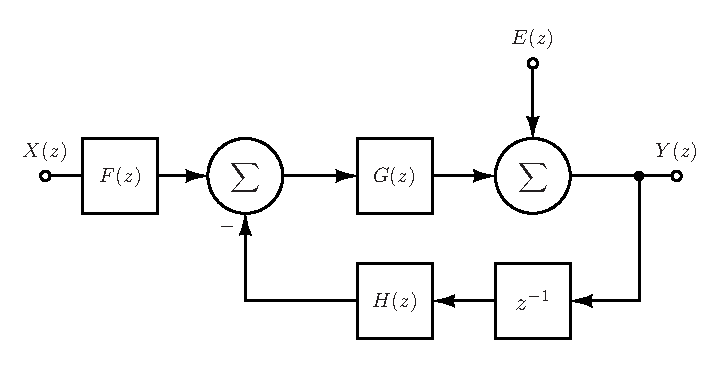
\includegraphics[width=0.7\textwidth]{DTDSM_lin}
	\end{figure}
	%---------------------------------------------------------------------------------
 	\vspace{-2mm}	
	\begin{equation*}
	Y(z)=\STF(z)X(z)+\NTF(z)E(z)
	\end{equation*}
	%---------------------------------------------------------------------------------
	\begin{equation*}
	\STF(z)=\frac{F(z)G(z)}{1+z^{-1}G(z)H(z)}\quad
	\NTF(z)=\frac{1}{1+z^{-1}G(z)H(z)}
	\end{equation*}
	\begin{itemize}
	\item Linearly modeled as a coupled set of complex transfer
	functions referred to as the Noise Transfer Function (NTF) and the Signal
	Transfer Function (STF)
	\end{itemize}
}

\onslide*{3}{
	\begin{large}
	Optimal Design of $\Delta\Sigma$ Modulator Data Converters 
	\end{large}
	%---------------------------------------------------------------------------------
 	\vspace{-3mm}
	%---------------------------------------------------------------------------------
	\begin{figure}[h!]
	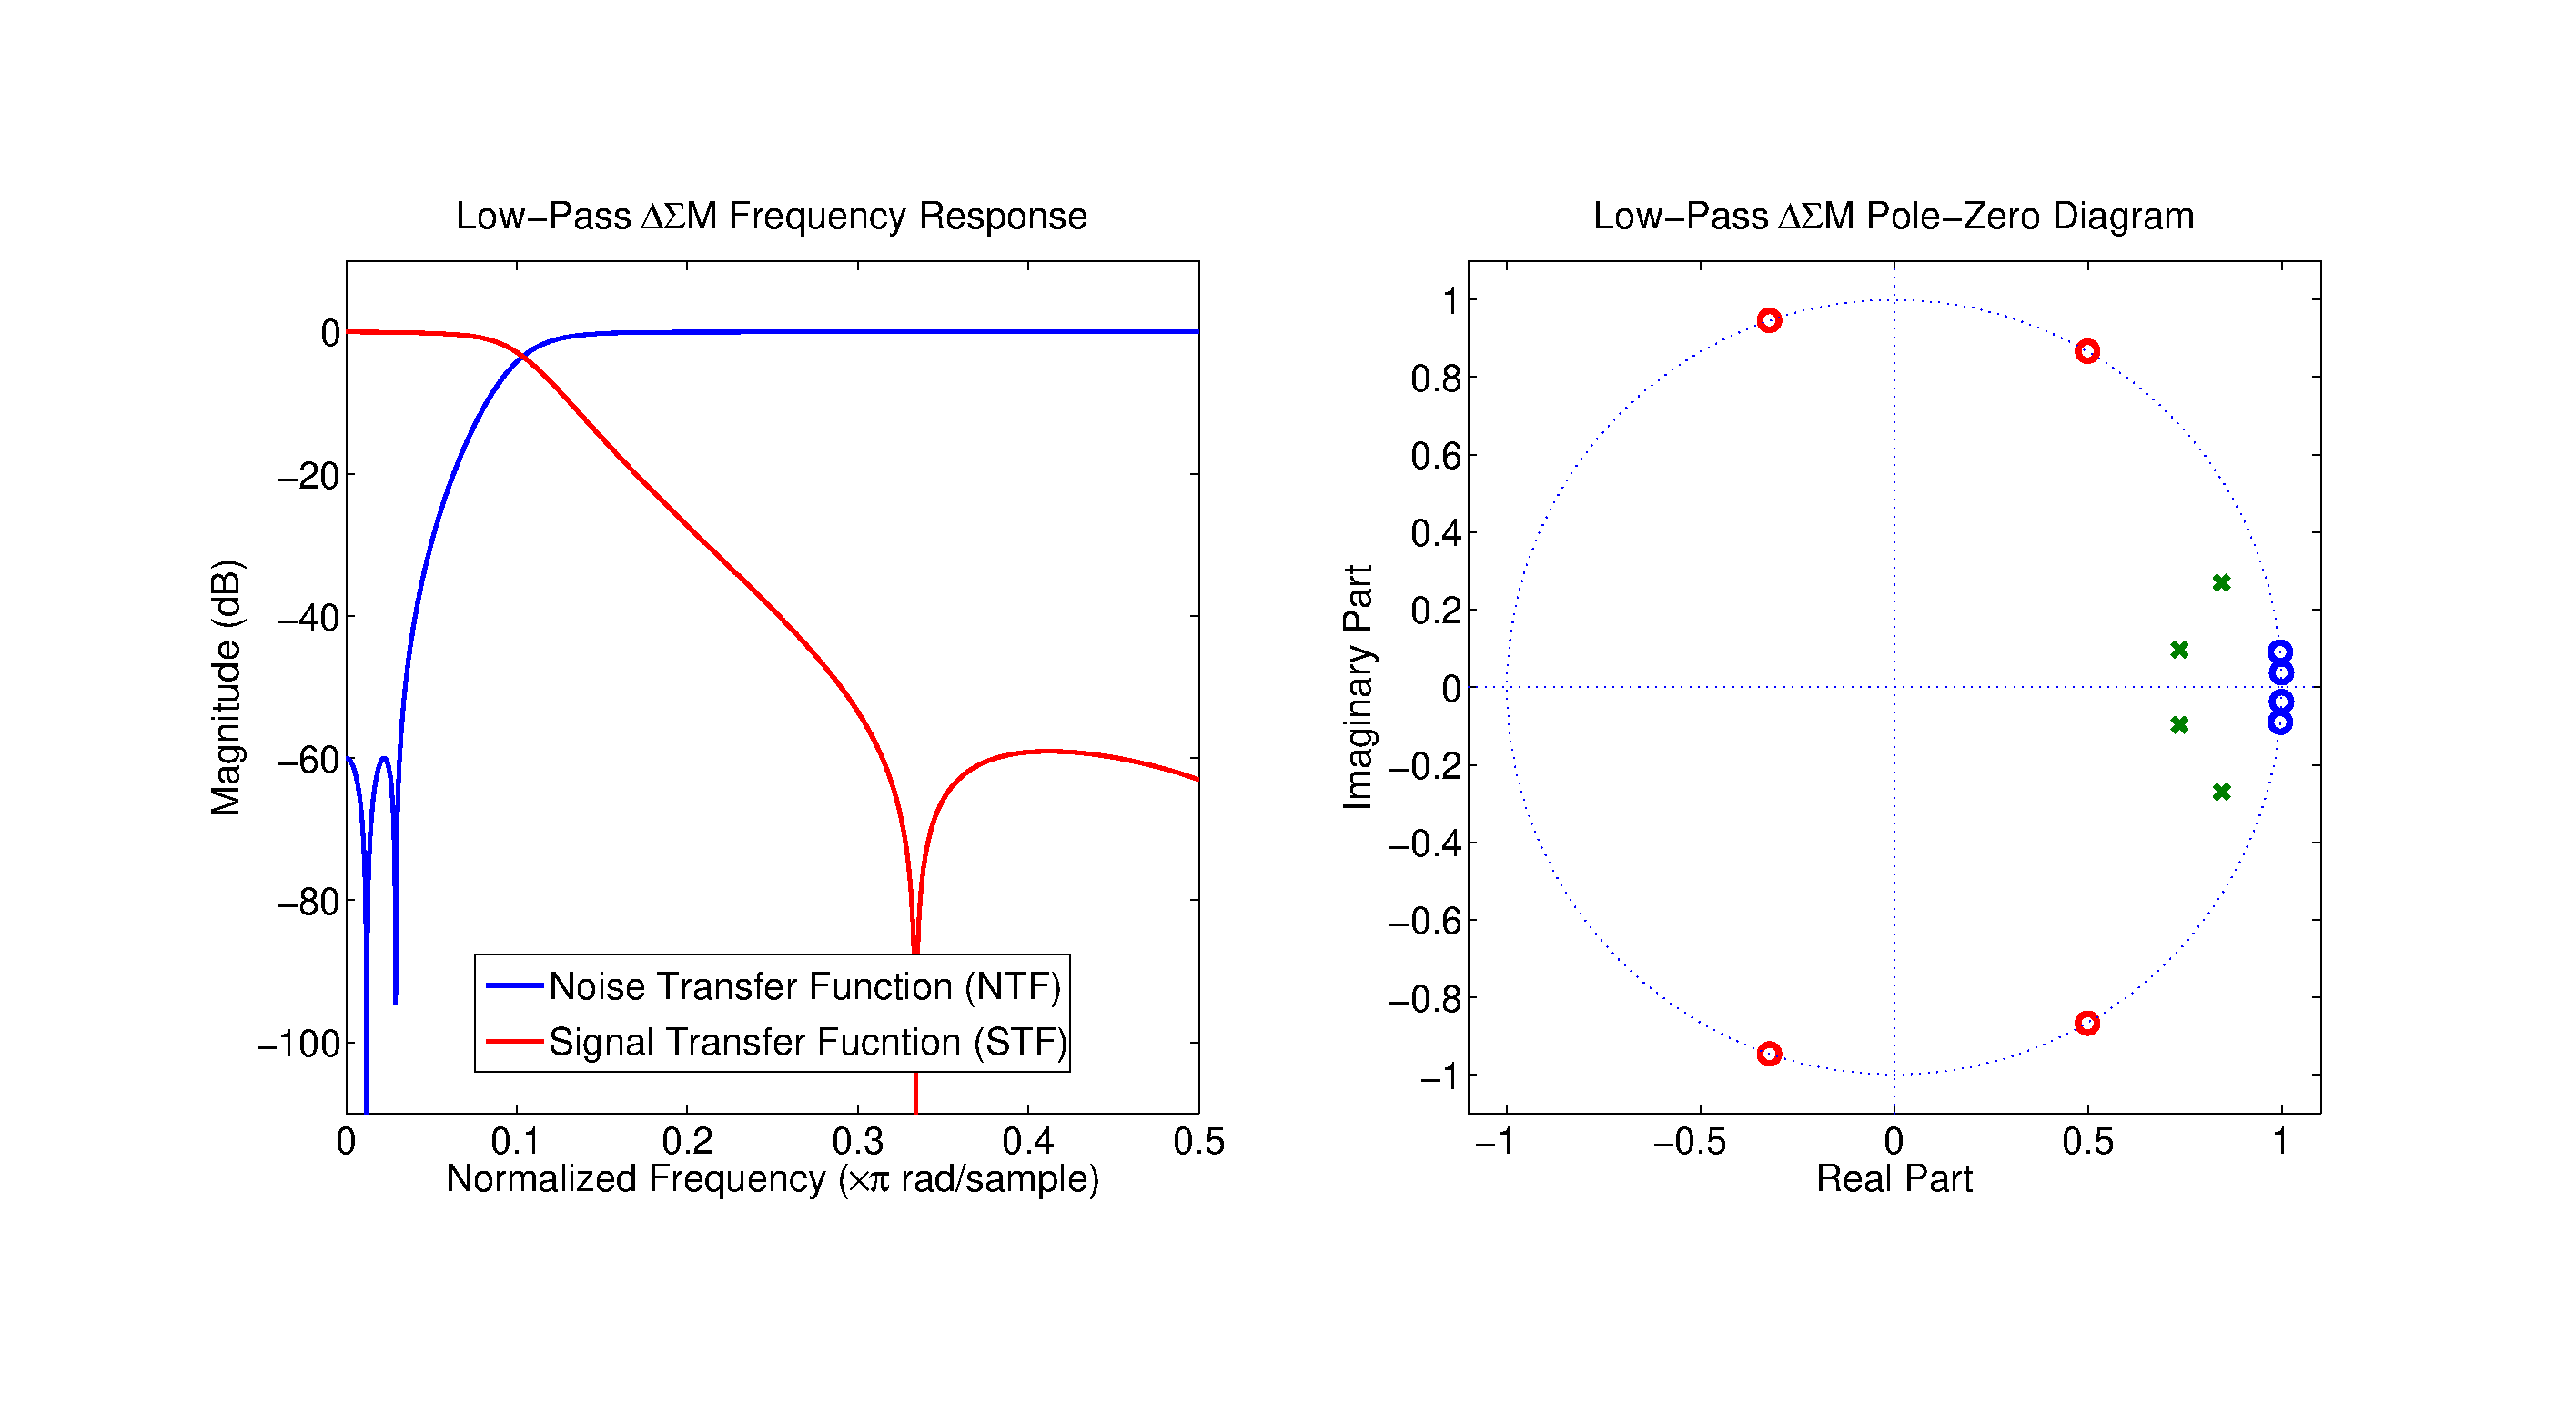
\includegraphics[width=0.925\textwidth]{DTDSM_freqs}
	\end{figure}
	%---------------------------------------------------------------------------------
	\vspace{-7mm}
	%---------------------------------------------------------------------------------
	\begin{itemize}
		\item Designed as a complimentary set of system functions such that the STF
		and NTF share common poles
		\item Classical Design Techniques: Chebyshev, Bessel, etc.
		\item EDA Based Methods: MATLAB DelSig Toolbox (R. Schreier)
	\end{itemize}
}
\end{slide}

%%%%%%%%%%%%%%%%%%%%%%%%%%%%%%%%

%%%%%%%%%%%%%%%%%%%%%%%%%%%%%%%%
%%% RATIONALE
\begin{slide}{Rationale}
	\begin{small}
 	\begin{itemize}[type=1]
  		\item \textbf{Problem Description:}\\ Optimal Design of Infinite Impulse Response
			  (IIR) Filters
		\begin{itemize}
			\item Minimize cost functions representing optimal filter performance
			\item Topic of interest since the late 1950s (Linear Programming)
			\item Multimodal performance surface
			\item Highly non-linear and non-differentiable \pause
		\end{itemize}
  		\item \textbf{Solution Techniques:} Constrained Global Optimization
  		\begin{itemize}
  			\item Linear / Non-Linear programming techniques
  			\item Directed search algorithms
  			\item Traditional genetic algorithms (GAs) and evolutionary strategies 
				  (ESs)
			\item Memetic GAs which employ second level learning to adaptively modify the
				  algorithm parameters \pause
  		\end{itemize}
  		\item \textbf{Proposed Solution:} Hybrid Orthogonal Genetic (HOG) Algorithm 
  		\begin{itemize}
  			\item Numerically reasonable global optimizer
  			\item Robust for complex performance surfaces
  			\item Flexible and easily adaptable for differing cost functions
  		\end{itemize}	
 	\end{itemize}
 	\end{small}
\end{slide}
%%%%%%%%%%%%%%%%%%%%%%%%%%%%%%%%

%%%%%%%%%%%%%%%%%%%%%%%%%%%%%%%%
%%% DTDSM OBJECTIVE FUNCTIONS
\begin{wideslide}[toc=Objective Functions,bm=Objective Functions]
{\DS Modulator Design Objective Functions}

\onslide*{1}{
\vfill
\centering
\textbf{Noise Transfer Function Objective Function}
%-----------------------
\begin{equation*}
J_{\NTF}=
\alpha\norm{\NTF(k)}^2_{\twosub{2}{k\in k_\text{sb}}}
+\beta\norm{\NTF(k)}_{\twosub{\infty}{k\in k_\text{sb}}}
+(1-\alpha-\beta)\norm{1-\lvert\NTF(k)\rvert}_{\twosub{1}{k\in k_\text{pb}}}
\end{equation*}
%-----------------------
\vfill
%-----------------------
\begin{itemize}
 \item Approximated by taking the DFT of the NTF frequency response
 \vfill
 \item Stopband error minimized wrt weighted combination of SNR and DR
 \vfill
 \item Passband error minimized to eliminate peaking
\end{itemize}
%-----------------------
\vfill
%-----------------------
\includegraphics*[clip,width=0.9\textwidth,viewport=0 0 475
175]{NTF_objective_fn.eps}
%-----------------------
\vfill \strut
}

\onslide*{2}{
\vfill
\centering
\textbf{Signal Transfer Function Objective Function}
%-----------------------
\begin{equation*}\label{eq:STF_objective_function}
J_{\STF}=
\zeta\norm{\STF(k)}^2_{\twosub{2}{k\in k_\text{sb}}}
+(1-\zeta)\norm{1-\lvert\STF(k)\rvert}_{\twosub{1}{k\in k_\text{pb}}}
\end{equation*}
%-----------------------
\vfill
%-----------------------
\begin{itemize}
 \item Approximated by taking the DFT of the STF frequency response
 \vfill
 \item Stopband error minimized to minimize out of band signal energy
 \vfill
 \item Passband error minimized to eliminate peaking
\end{itemize}
%-----------------------
\vfill
%-----------------------
\includegraphics*[clip,width=0.9\textwidth,viewport=0 0 475
175]{STF_objective_fn.eps}
%-----------------------
\vfill \strut
}

\end{wideslide}
%%%%%%%%%%%%%%%%%%%%%%%%%%%%%%%%

%%%%%%%%%%%%%%%%%%%%%%%%%%%%%%%%%%%%%%%%%%%%%%%%%%%%%%%%%%%%%%%%%%%%%%%%%%%%%%%%
%% GENETIC ALGORITHMS
%%%%%%%%%%%%%%%%%%%%%%%%%%%%%%%%%%%%%%%%%%%%%%%%%%%%%%%%%%%%%%%%%%%%%%%%%%%%%%%%
\section[toc=HOG Algorithm,bm=HOG Algorithm]{Hybrid Orthogonal Genetic (HOG) Algorithm}

%%%%%%%%%%%%%%%%%%%%%%%%%%%%%%%%
%%% GENETIC ALGORITHMS: OVERVIEW
\begin{slide}[toc=GA Overview,bm=GA Overview]{Genetic Algorithms: Overview}
	\twocolumn{
	\strut \vfill
% 	\begin{center}
		\begin{itemize}[type=1]
 			\item General Theory \pause
 			\vspace{2mm}
			\item Population Initialization\pause
 			\vspace{2mm}
			\item Fitness Evaluation\pause
 			\vspace{2mm}
			\item Progenitor Selection\pause
 			\vspace{2mm}
			\item Reproduction\pause
 			\vspace{2mm}
			\item Genetic Diversity\pause
 			\vspace{2mm}
			\item Convergence
		\end{itemize}
% 	\end{center}
	\vfill \strut
	}
	{
	\centering
	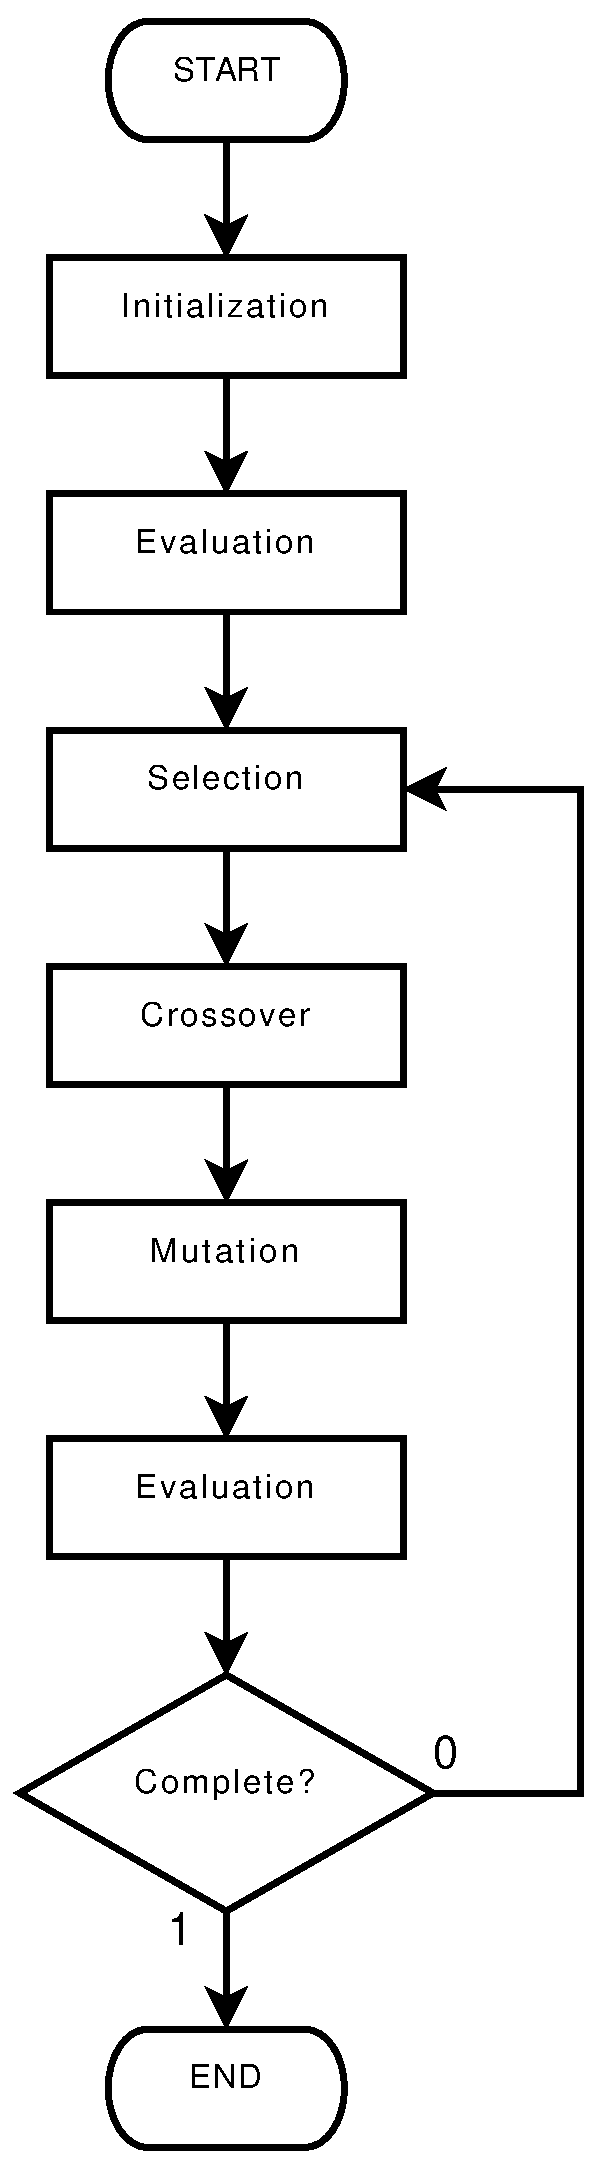
\includegraphics[height=7.75cm]{simple_ga_flow}
	}
\end{slide}
%%%%%%%%%%%%%%%%%%%%%%%%%%%%%%%%

%%%%%%%%%%%%%%%%%%%%%%%%%%%%%%%%
%%% HYBRID ORTHOGONAL GENETIC ALGORITHM
\begin{slide}[toc=HOG Overview,bm=HOG Overview]{HOG Algorithm Overview}
	\twocolumn[\savevalue{lcolwidth} = 5cm, rcolwidth = 5.6cm, colsep = -0.25cm]{
		\vspace{2cm}
		\begin{itemize}[type=1]
			\item Linear-Ranking Selection
			\vspace{2mm}
			\item Single-Point Crossover
			\vspace{2mm}
			\item Orthogonal Crossover
			\vspace{2mm}
			\item Point-Swap Mutation
		\end{itemize}
		}
	{
		\centering
		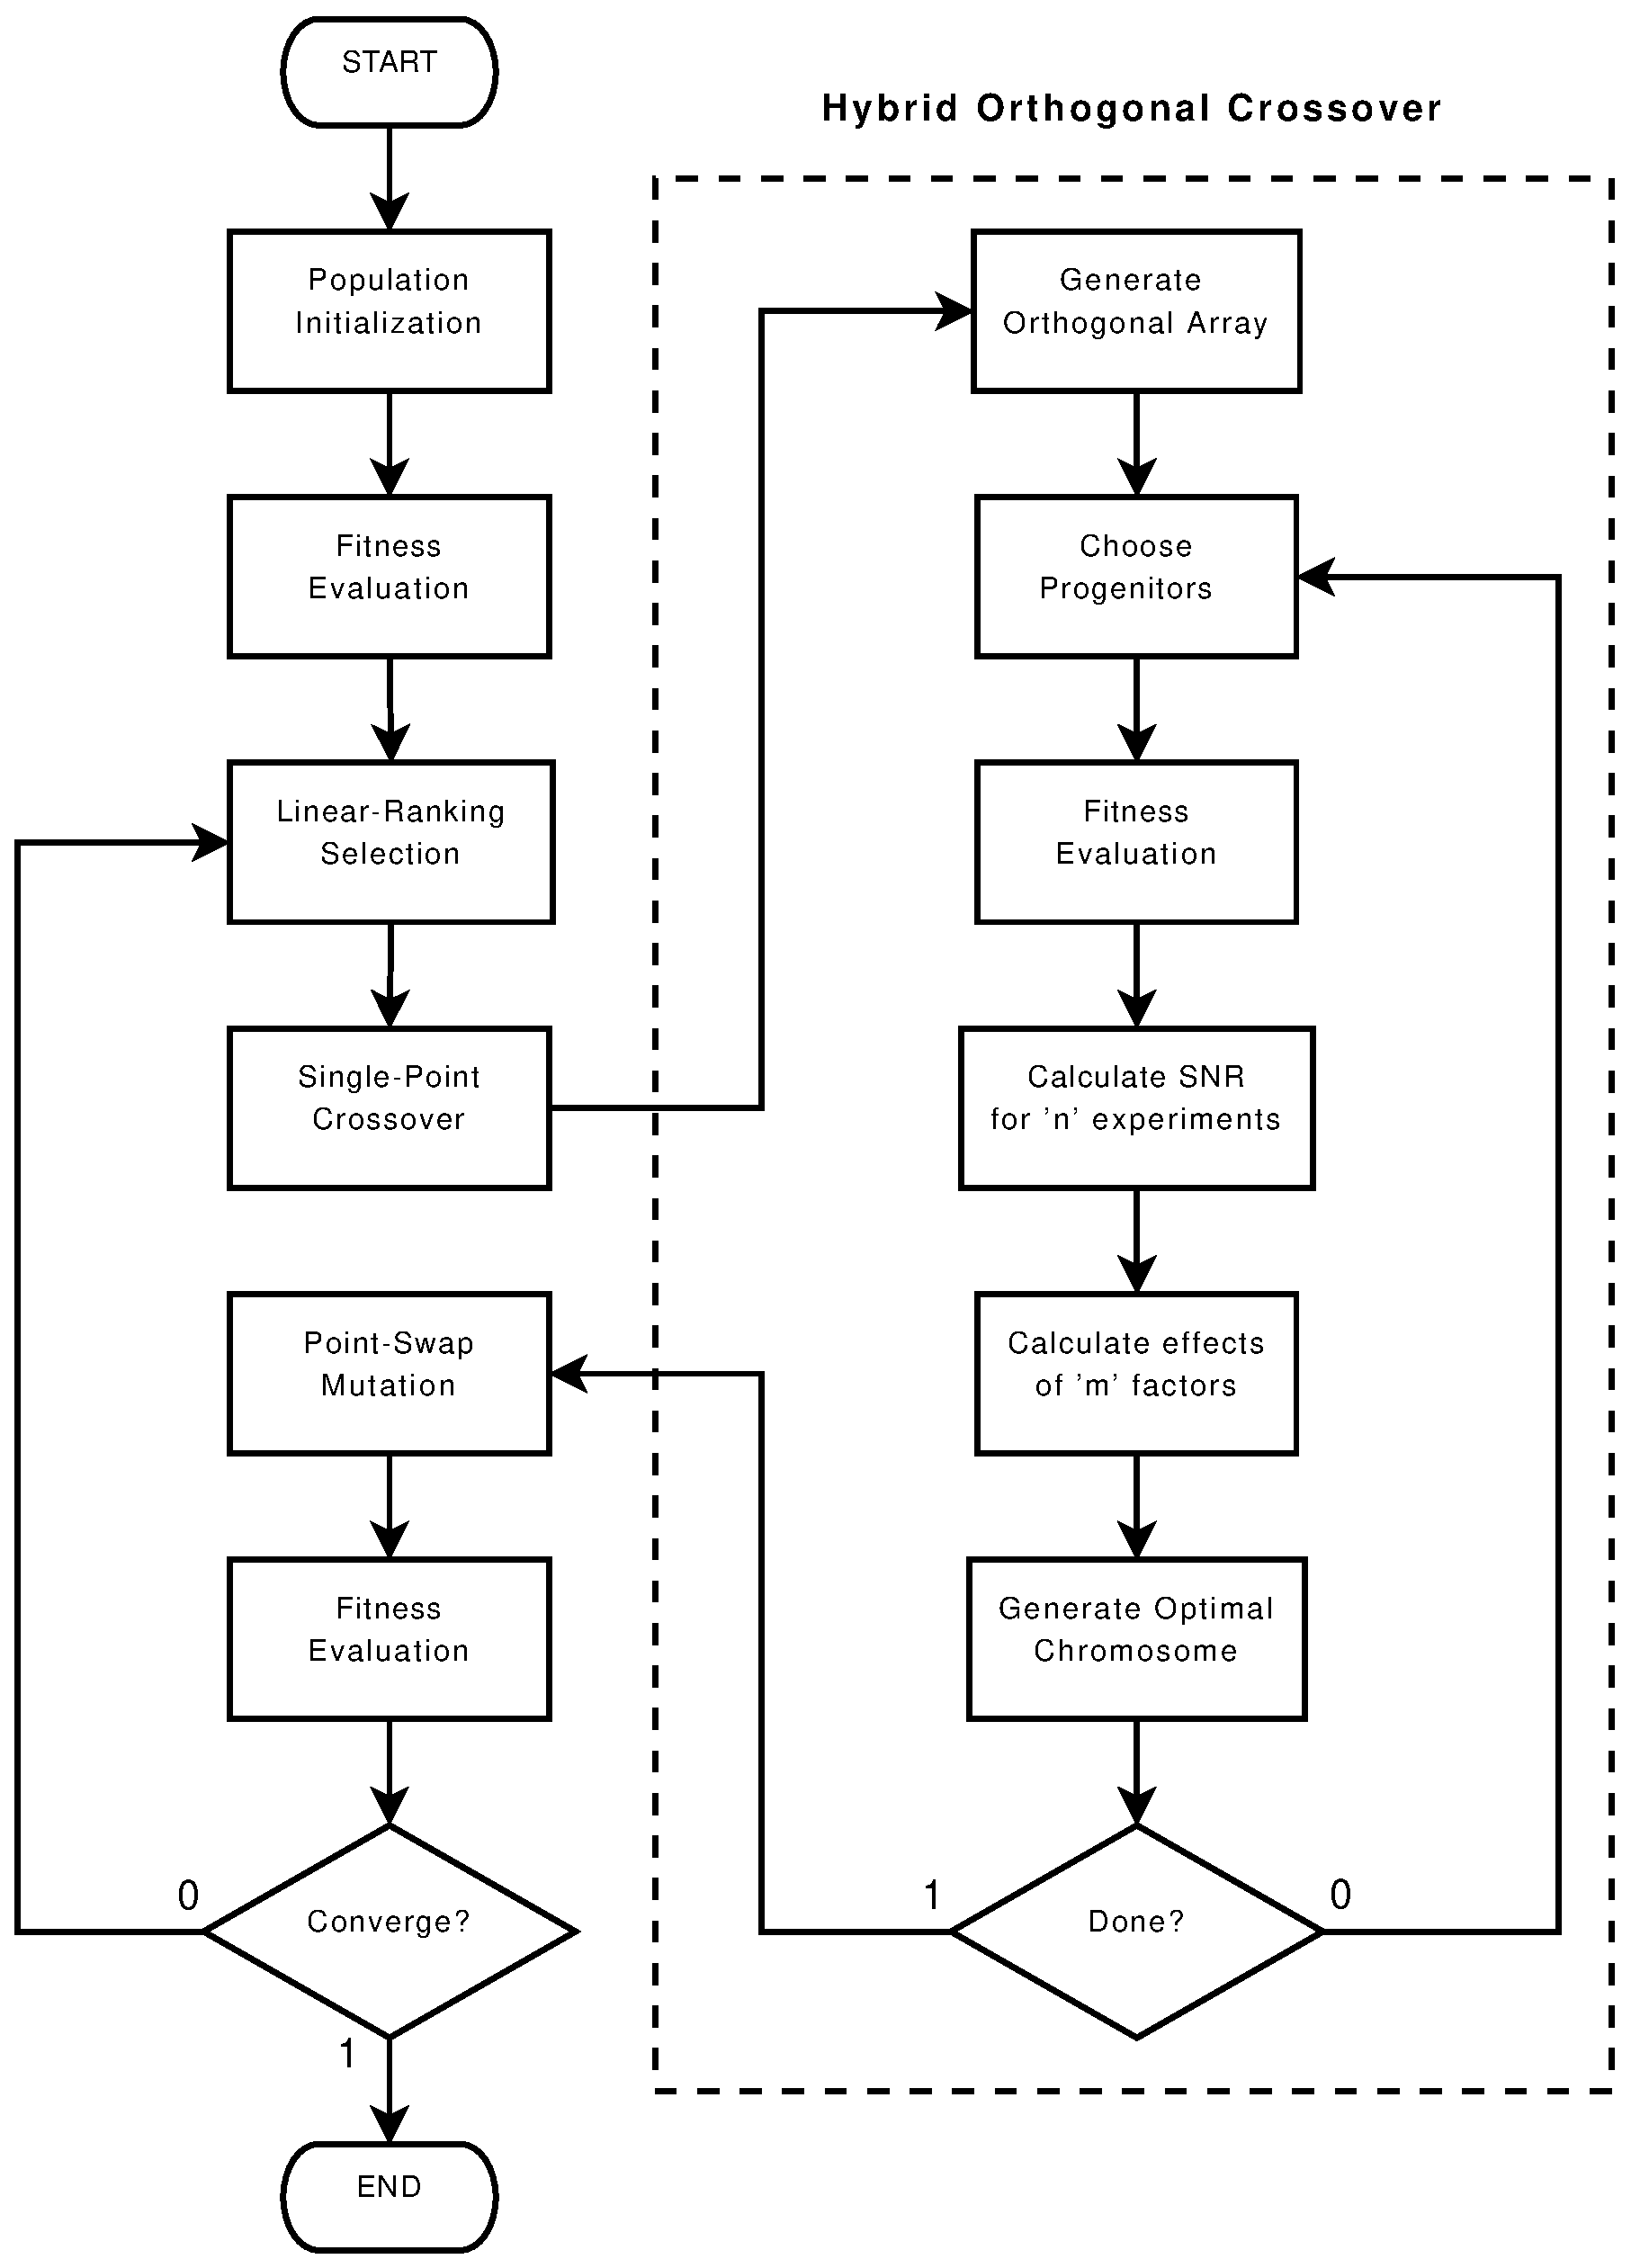
\includegraphics[height=7.75cm]{HOGA_flow}
	}
\end{slide}
%%%%%%%%%%%%%%%%%%%%%%%%%%%%%%%%

% %%%%%%%%%%%%%%%%%%%%%%%%%%%%%%%%
% %%% INITIALIZATION AND EVALUATION
% \begin{slide}[toc=Population,bm=Population]{Population Initialization and Evaluation}
%
%----------------------------------------------------------------------------------------
% Population Initialization
% \begin{itemize}
%  \item Distinct members referred to as chromosomes
%  \item Exploration of unknown performance surfaces
%  \item Exploitation of known performance surfaces
%  \item Feasible region constraints
% \end{itemize}
% \vspace{5mm}
% Fitness Evaluation
% \begin{equation*}\label{eq:objective_function}
%  J_{x}=\min_{x\in\mathbb R}\bigl\{f(x)\bigr\}
% \quad \forall x \in \mathbb{R}^N
% \end{equation*}\begin{itemize}
%  \item Minimization of the objective (cost) function
%  \item Each chromosome evaluated for fitness against the objective (cost) function
% \end{itemize}
%
%----------------------------------------------------------------------------------------
% \end{slide}
% %%%%%%%%%%%%%%%%%%%%%%%%%%%%%%%%

%%%%%%%%%%%%%%%%%%%%%%%%%%%%%%%%
%%% LINEAR-RANKING SELECTION
\begin{slide}[toc=Selection,bm=Selection]{Linear-Ranking Selection}
	\vfill
	\textbf{Theory}
	\begin{itemize}
 		\item Mating eligibility is a function of relative fitness and \textit{selection
		pressure}
		\vfill
		\begin{itemize}
			\item Least-fit probability of selection:$\bigl(\eta^{-}/N\bigr)$ 
			\vfill
			\item Most-fit probability of selection: $\bigl(\eta^{+}/N\bigr)$
		\end{itemize}
	\end{itemize}
	$$\eta^{-}=2-\eta^{+}$$
	\vfill

	\textbf{Implementation}
	\begin{itemize}
		\item Sorted and ranked according to relative fitness from least to greatest
		\vfill
		\item Assigned an integer index value $i\in[0,N-1]$
		\vfill
		\item Assigned a probability of selection according to
		\vfill
%  		\vspace{-2.5mm}
	\end{itemize}
 	\begin{equation*}
		p_{i}=\frac{1}{N}\biggl(\eta^{-}+\bigl(\eta^{+}-\eta^{-}\bigr)
		\frac{i-1}{N-1}\biggr)
	\end{equation*}
	\vfill \strut
\end{slide}
%%%%%%%%%%%%%%%%%%%%%%%%%%%%%%%%

%%%%%%%%%%%%%%%%%%%%%%%%%%%%%%%%
%%% SINGLE-POINT CROSSOVER OPERATOR
\begin{slide}[toc=Crossover,bm=Crossover]{Single-Point Crossover Operator}
	\vfill
% 	\vspace{-5mm}
	\centering
	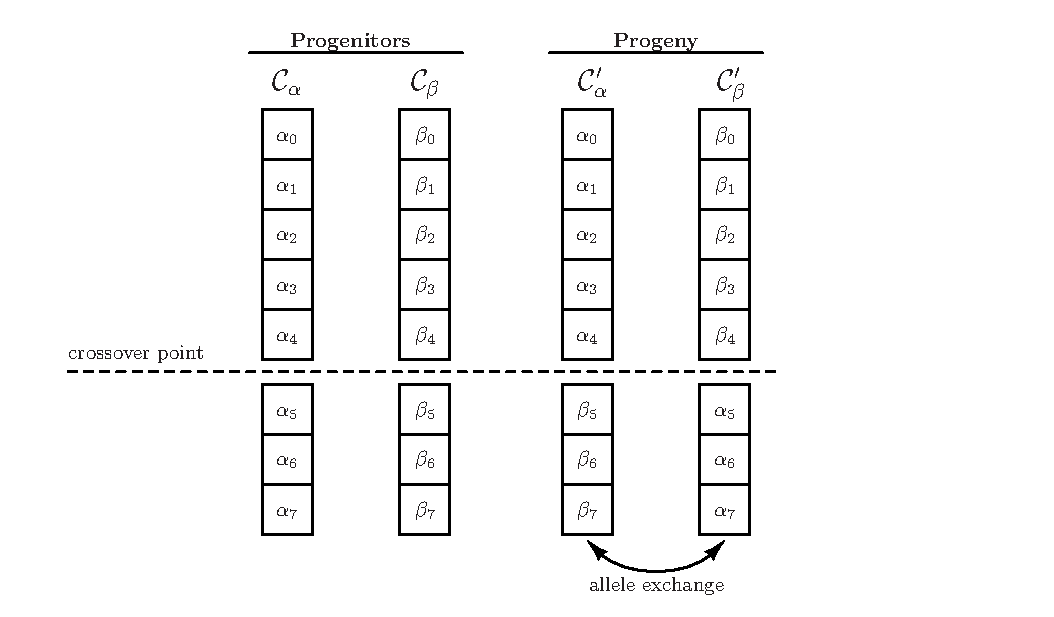
\includegraphics[height=5cm]{crossover}
	\vfill
	\begin{itemize}
 		\item Pairs of progenitors are randomly selected from the mating pool and assigned
		a random number, $r$, which is uniform over $\bigl[0,1\bigr]$
		\vfill
 		\item For $r\geq P_c$: crossover occurs and genetic information is exchanged
 		\vfill
  		\item If crossover occurs, a discrete random number, $c$, uniform over
		$\bigl[0,m\bigr]$ is picked to determine the crossover point
	\end{itemize}
	\vfill \strut
\end{slide}
%%%%%%%%%%%%%%%%%%%%%%%%%%%%%%%%

%%%%%%%%%%%%%%%%%%%%%%%%%%%%%%%%
%%% POINT-SWAP MUTATION OPERATOR
\begin{slide}[toc=Mutation,bm=Mutation]{Point-Swap Mutation Operator}
	\vfill
	\centering
	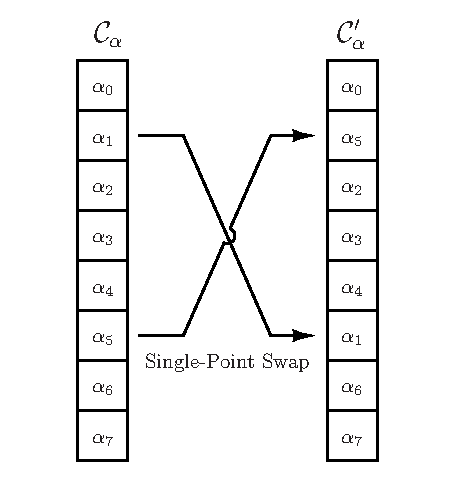
\includegraphics[height=4.2cm]{single_point_mutation}
	\vfill
	\begin{itemize}
		\item Individual chromosomes are randomly selected from the population
		\vfill
		\item Selected chromosome is assigned a random number, $s$, which is uniform over
		$\bigl[0,1\bigr]$
		\vfill
		\item For $s\geq P_m$: mutation occurs and new genetic information is created
		\vfill
		\item Mutation occurs \textit{unbounded}
	\end{itemize}
	\vfill \strut
\end{slide}
%%%%%%%%%%%%%%%%%%%%%%%%%%%%%%%%

%%%%%%%%%%%%%%%%%%%%%%%%%%%%%%%%
%%% TAGUCHI METHOD
\begin{slide}[toc=Taguchi Method,bm=Taguchi Method]
{Hybrid Orthogonal Crossover via the Taguchi Method}

\onslide*{1}{
	\vfill
	\textbf{Theory}
	\begin{itemize}
		\item Crossover and subsequent fitness evaluation can be viewed as performing
		experiments on the population
		\vfill
		\item Design of experiments (DoE) statistical techniques can be implemented
		to minimize the number of trials required to observe the effects of the
		experimental factors
	\end{itemize}
	\vfill
	
	\textbf{Implementation}
	\begin{itemize}
		\item Pairs of progenitors are randomly selected from the population whose
		respective traits become the \textit{experimental factors}
		\vfill
		\item The factors are mapped to an appropriately sized orthogonal array and the
		effects for each factor are observed via a metric, $S$
		\vfill
		\item Optimal offspring are created from the most beneficial factors
	\end{itemize}
	\vfill \strut
}

\onslide*{2}{
	\textbf{Orthogonal Arrays (OAs)}
		\begin{itemize}
		\item Derived from Latin Squares (e.g. Sudoku)
		\vfill
		\item Taguchi Method uses 2-Level OAs of the form $L_n\bigl(2^{n-1}\bigr)$
		\vfill
		\item Number of Trials: $n$
		\vfill
		\item Number of Factors: $n-1$
		\vfill
	\end{itemize}
	\begin{equation*}
		\text{OA Example for 4 trials/3 factors:}\qquad
 		L_4\bigl(2^{3}\bigr)=
		\begin{pmatrix}
			1 &1 &1 \\
			1 &2 &2 \\
			2 &1 &2 \\
			2 &2 &1 \\
		\end{pmatrix}
	\end{equation*}
	\vfill
	
	\begin{itemize}
		\item OA elements directly control mapping of factors from a particular
		progenitor to the experimental matrix
		\vfill
		\item Each column representing a factor is independent from the other columns
	\end{itemize}
	\vfill \strut
}

\onslide*{3}{
	\vfill
	\textbf{Taguchi Metric} ($S_n$)
	\begin{equation*}
		S_n=J^{2}(\bm{x}_n)
	\end{equation*}
	\vfill
	%---------------------------------------------------------------------------------
	\begin{itemize}
		\item Objective function evaluation squared for $n$ experimental
		trials (e.g. each row of the 2-level OA)
		\vfill
		\item $\bm{x}_n$ is a vector containing the $k$ factors of the $n$th trial
		\vfill
		\item Smaller-is-better calculation for global minimization
	\end{itemize}
	%---------------------------------------------------------------------------------
	\vfill
	\textbf{Optimal Progeny Generation}
	\begin{equation*}
		E_{x_{k}P_{m}}=\sum_{i\in \{k:x_k = P_m\}}S_i
	\end{equation*}
	\vfill
	\begin{itemize}
		\item Effects, $E$, from all $k$ factors from each progenitor, $P_1$ and $P_2$,
		evaluated based on the metric, $S$
		\vfill
		\item Factor with best observed effect populates the optimal progeny
		\vfill
		\item Generates optimal offspring from the available progenitors
	\end{itemize}
	\vfill \strut
}

\end{slide}
%%%%%%%%%%%%%%%%%%%%%%%%%%%%%%%%

\section{HOG Algorithm Examples}

%%%%%%%%%%%%%%%%%%%%%%%%%%%%%%%%
%%% EXAMPLE: MATLAB PEAKS FUNCTION
\begin{wideslide}[toc=MATLAB Peaks,bm=MATLAB Peaks]
{Example: MATLAB Peaks Function}
	\vfill
		\begin{equation*}
 			P(x,y)=
			3\left(1-x\right)^2
			e^{\left(-x^{2}-\left(y+1\right)^{2}\right)}-
			10\left(\frac{x}{5}-x^{3}-y^{5}\right)e^
			{\left(-x^{2}-y^{2}\right)}-
			\frac{1}{3}e^{\left(-\left(x+1\right)^{2}-y^{2}\right)}
		\end{equation*}
	\vfill
	\centering
	%---------------------------------------------------------------------------------
	\begin{figure}[htbp]
	\subfigure{
	\includegraphics[,width=0.225\slidewidth,clip,viewport=320 50 1040
725]{peaks_surf}
	}
	\subfigure{
	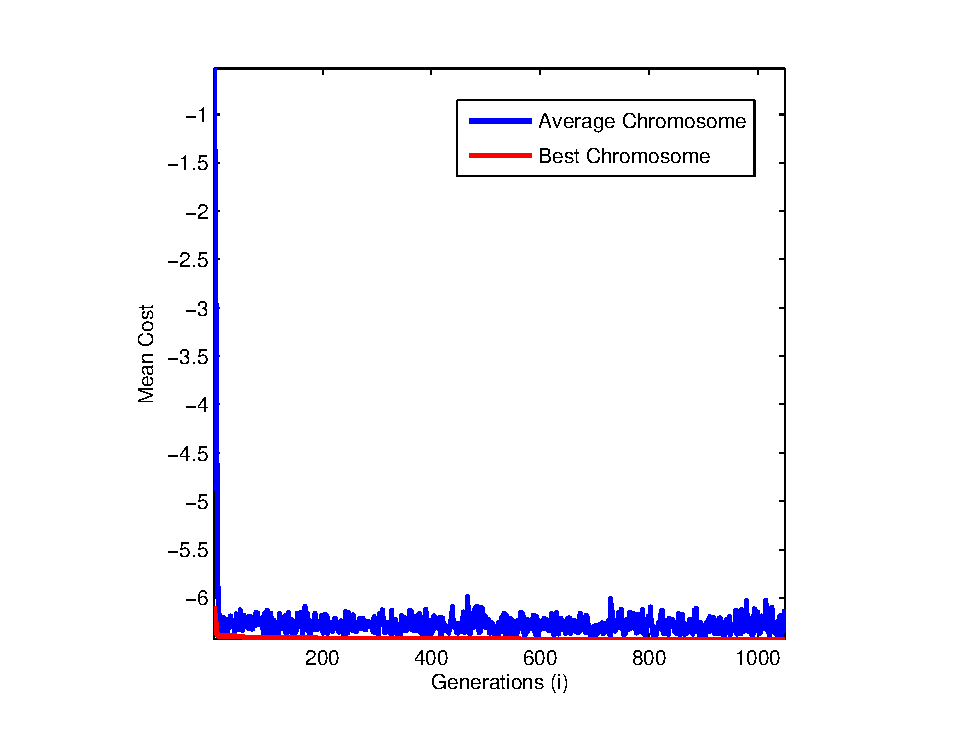
\includegraphics[width=0.3\slidewidth]{peaks_learning_curve}
	}
	\subfigure{
	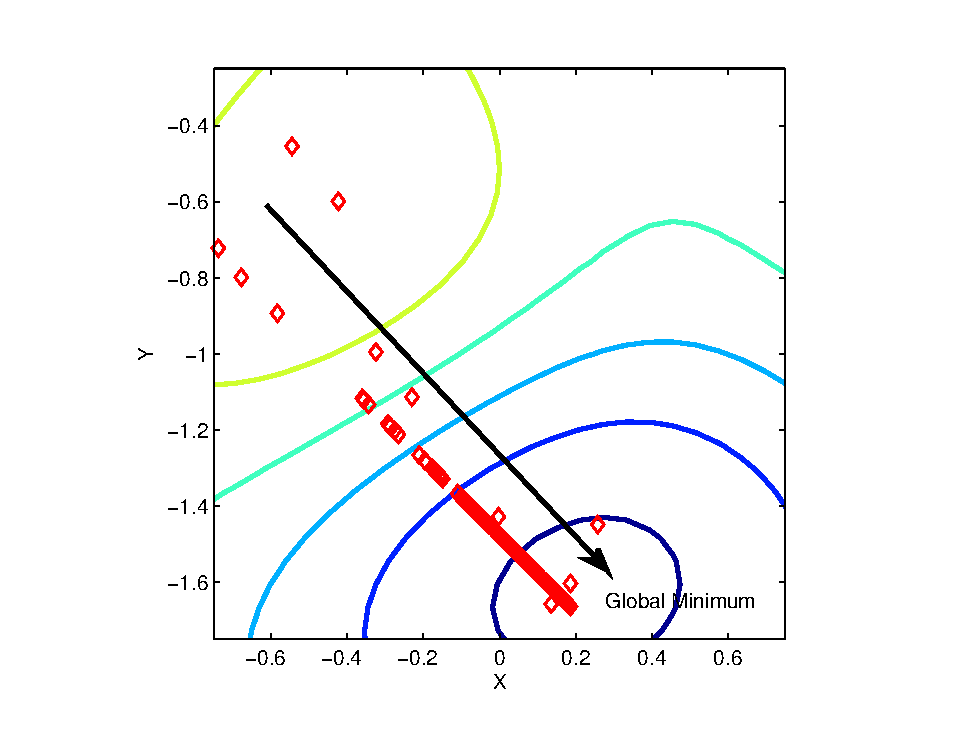
\includegraphics[width=0.3\slidewidth]{peaks_descent}
	}
	\end{figure}
	%---------------------------------------------------------------------------------
	\vfill
	\begin{itemize}
 		\item Obtained by translating and scaling Gaussian distributions
 		\vspace{1mm}
 		\item 2 local minima and 1 global minimum near $(0.2,-1.625)$
 		\vspace{1mm}
 		\item Quick convergence
		\vspace{1mm}
		\item Resembles steepest descent convergence path
	\end{itemize}
	\vfill \strut
\end{wideslide}
	


%%%%%%%%%%%%%%%%%%%%%%%%%%%%%%%%
%%% EXAMPLE: RASTRIGIN'S FUNCTION
\begin{wideslide}[toc=Rastrigin,bm=Rastrigrin]{Example: Rastrigin's Function}
	\vfill
	\begin{equation*}
 		f(x) = \sum_{i=1}^{N}\Bigl[x_{i}^2-10\cos\bigl(2\pi x_i\bigr)+10\Bigr]\quad
		\forall x \in \mathbb{R}^N
	\end{equation*}
	\vfill
	\centering
	%---------------------------------------------------------------------------------
	\begin{figure}[htbp]
	\subfigure{
	\includegraphics[,width=0.225\slidewidth,clip,viewport=320 50 1040
725]{rast_surf}
	}
	\subfigure{
	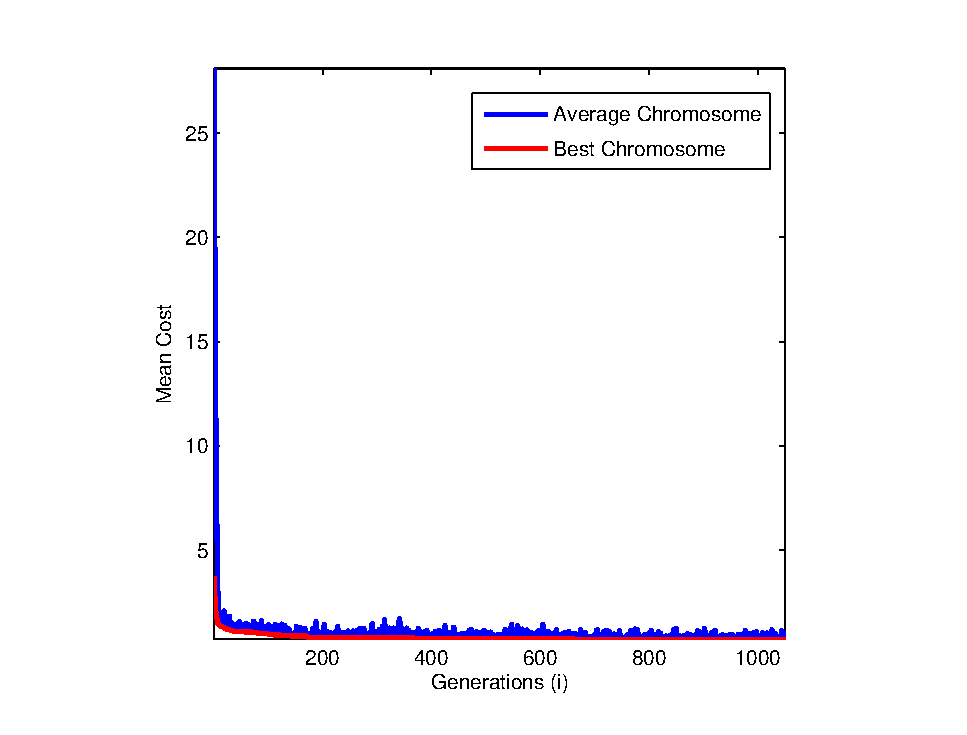
\includegraphics[width=0.3\slidewidth]{rast_learning_curve}
	}
	\subfigure{
	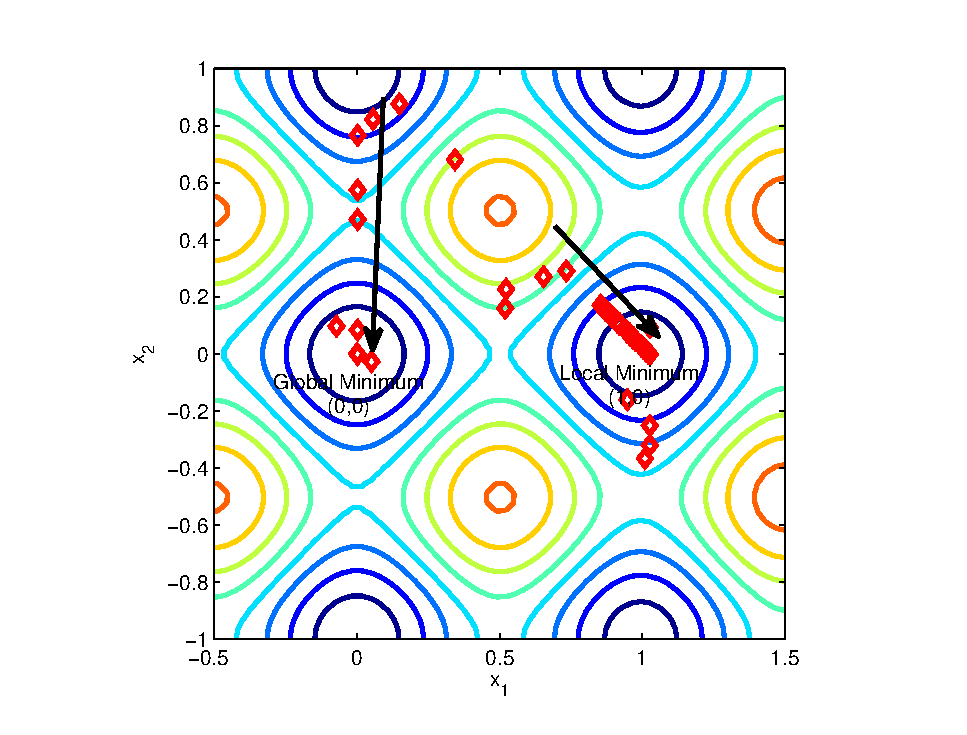
\includegraphics[width=0.3\slidewidth]{rast_descent}
	}
	\end{figure}
	%---------------------------------------------------------------------------------
	\vfill
	\begin{itemize}
 		\item Widely accepted global optimization algorithm test function
  		\vspace{1mm}
 		\item Characterized by a parabolic egg-crate shape with single lowest point
		\vspace{1mm} 
 		\item Highly multimodal with a global minimum of $f(0,0) = 0$ for $\mathbb{R}^2$
		\vspace{1mm}
		\item Numerous local minima provides challenging performance surface
	\end{itemize}
	\vfill \strut
\end{wideslide}

%%%%%%%%%%%%%%%%%%%%%%%%%%%%%%%%
%%% EXAMPLE: ROSENBROCK'S BANANA FUNCTION
\begin{wideslide}[toc=Rosenbrock,bm=Rosenbrock]{Example: Rosenbrock's Function}
	\vfill
	\begin{equation*}
 		f(x) = \sum_{i=1}^{N-1}\Bigl[\bigl(1-x_i\bigr)^2+ 100 \bigl(x_{i+1} - x_i^2
		\bigr)^2\Bigr]\quad \forall x \in \mathbb{R}^N
	\end{equation*}
	\vfill
	\centering
	%---------------------------------------------------------------------------------
	\begin{figure}[htbp]
	\subfigure{
	\includegraphics[,width=0.225\slidewidth,clip,viewport=320 50 1040
725]{rose_surf}
	}
	\subfigure{
	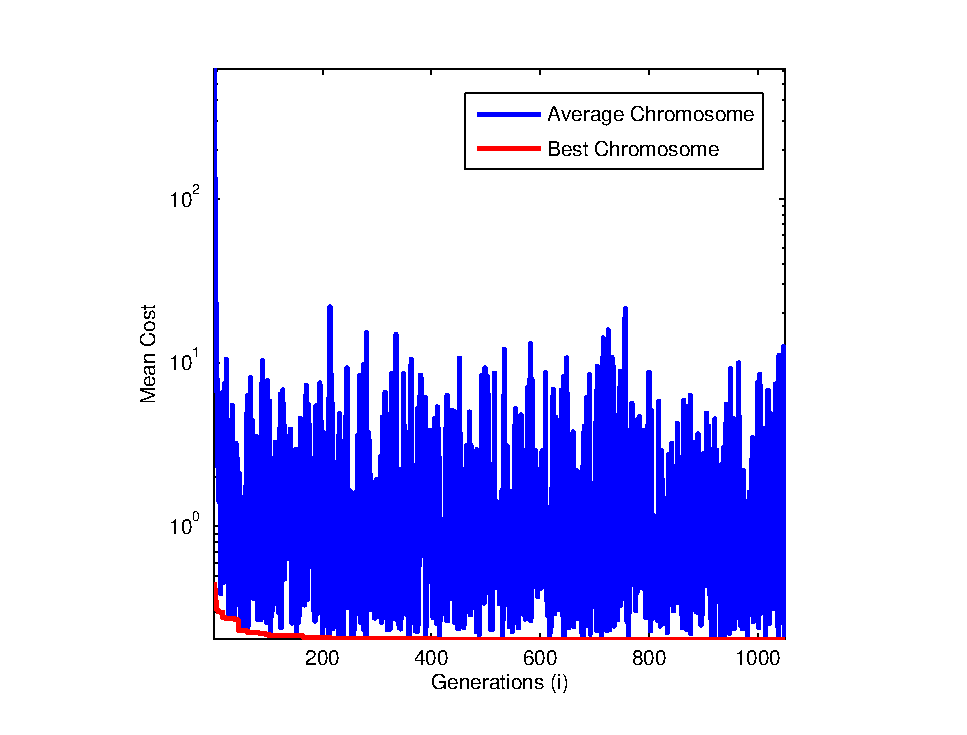
\includegraphics[width=0.3\slidewidth]{rose_learning_curve}
	}
	\subfigure{
	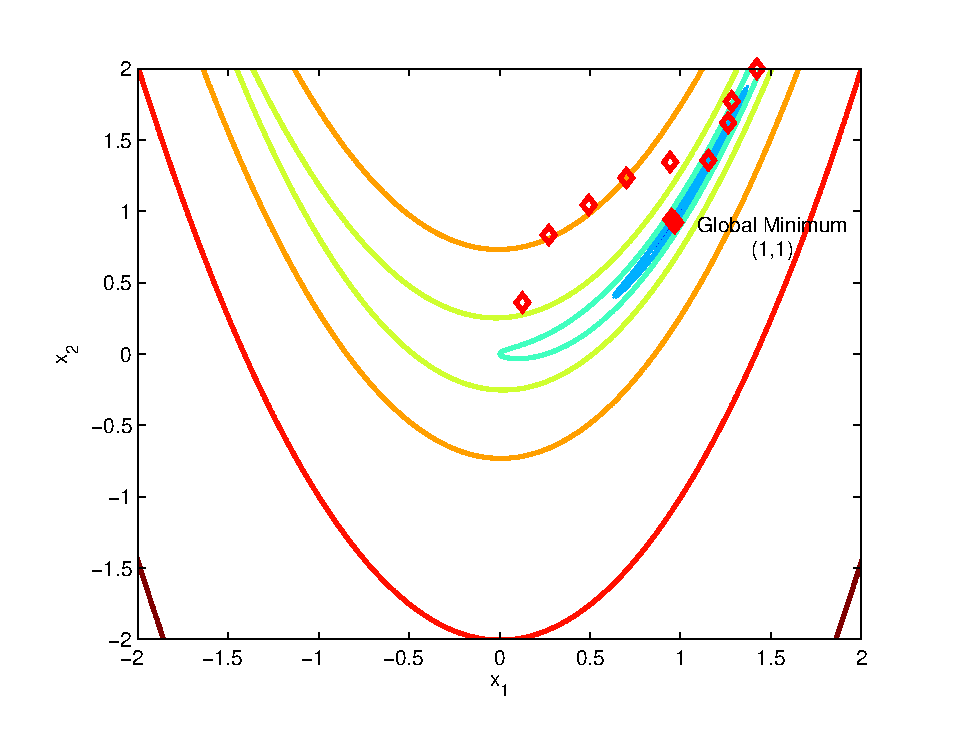
\includegraphics[width=0.3\slidewidth]{rose_descent}
	}
	\end{figure}
	%---------------------------------------------------------------------------------
	\vfill
	\begin{itemize}
 		\item Characterized by a steep parabolic ravine (banana) and gradual descent to
		global minimum
		\vspace{1mm} 
 		\item Unimodal with a global minimum of $f(1,1) = 0$ for $\mathbb{R}^2$
		\vspace{1mm}
		\item Long descent proves challenging for most algorithms
	\end{itemize}
	\vfill \strut
\end{wideslide}

%%%%%%%%%%%%%%%%%%%%%%%%%%%%%%%%
\section{DSM Design and Results}
%%%%%%%%%%%%%%%%%%%%%%%%%%%%%%%%

%% HOG Implementation
\begin{wideslide}[toc=HOG Implementation,bm=HOG Implementation]
{HOG Algorithm Implementation}

\onslide*{1}{
	\vfill
	\centering
	%---------------------------------------------------------------------------------
	\begin{equation*}
		\NTF(z)=\psi_N\biggl(\frac{1-a_1 z^{-1}}{1-b_1 z^{-1}}\biggr)^m
		\displaystyle\prod_{n=1}^{M}\frac{\bigl(1+c_{1n}z^{-1}+c_{2n}z^{-2}\bigr)}
		{\bigl(1+d_{1n}z^{-1}+d_{2n}z^{-2}\bigr)}
	\end{equation*}
	%---------------------------------------------------------------------------------
	\begin{itemize}[labelindent=0.18\slidewidth]
		\item Cascade of second-order sections (SOS)
		\vfill
		\item Reduces coefficient sensitivity to perturbation
	\end{itemize}
	\hrulefill
	\vfill
	%---------------------
	\begin{equation*}
		\mathcal{C}_{\text{NTF}} =
		\left[a_1,b_1,c_{11},c_{12},d_{11},d_{12},c_{21},c_{22},d_{ 21},
		d_{22},\dotsc,c_{M1},c_{M2},d_{M1},d_{M2},\psi_N\right]^T
	\end{equation*}
	%---------------------
	\vfill
	\hrulefill
	%---------------------	
	\begin{equation*}
		\mathbb{G}_{\text{NTF}}
		=\Bigl[\mathcal{C}_{\text{NTF},1}\dashline\mathcal{C}_{\text{NTF},2}
		\dashline\dotsb\dashline\mathcal{C}_{\text{NTF},n}\Bigr]
	\end{equation*}
	%---------------------
	\begin{itemize}[labelindent=0.1\slidewidth]
		\item Population matrix, $\mathbb{G}$, is an aggregate of $n$ chromosomes,
			  $\mathcal{C}$
	\end{itemize}
	%---------------------
	\vfill \strut
}

\onslide*{2}{
	\vfill
	\centering
	%---------------------------------------------------------------------------------
	\begin{equation*}
 		\STF(z)=\psi_S\biggl(\frac{1-\rho_1 z^{-1}}{1-b_1 z^{-1}}\biggr)^m
		\displaystyle\prod_{n=1}^{M}\frac{\bigl(1+\nu_{1n}z^{-1}+\nu_{2n}z^{-2}\bigr)}
		{\bigl(1+d_{1n }z^{-1}+d_{2n}z^{-2}\bigr)}
	\end{equation*}
	%---------------------------------------------------------------------------------
	\begin{itemize}[labelindent=0.18\slidewidth]
		\item Cascade of second-order sections (SOS)
		\vfill
		\item Reduces coefficient sensitivity to perturbation
	\end{itemize}
	\hrulefill
	\vfill
	%---------------------
	\begin{equation*}
		\mathcal{C}_{\text{STF}} =
		\left[\rho_1,\nu_{11},\nu_{12},\nu_{21},\nu_{22},\dotsc,\nu_{M1},\nu_{M2},
		\psi_S\right]^T
	\end{equation*}
	%---------------------
	\vfill
	\hrulefill
	%---------------------	
	\begin{equation*}
		\mathbb{G}_{\text{STF}}
		=\Bigl[\mathcal{C}_{\text{STF},1}\dashline\mathcal{C}_{\text{STF},2}
		\dashline\dotsb\dashline\mathcal{C}_{\text{STF},n}\Bigr]
	\end{equation*}
	%---------------------
	\begin{itemize}[labelindent=0.1\slidewidth]
		\item Population matrix, $\mathbb{G}$, is an aggregate of $n$ chromosomes,
			  $\mathcal{C}$
	\end{itemize}
	%---------------------
	\vfill \strut
}
\end{wideslide}




%% Modeling
\begin{slide}[toc=Modeling,bm=Modeling]{LTI System Modeling}

\onslide*{1}{
	\centering
	%---------------------------------------------------------------------------------
	\begin{figure}[h!]
	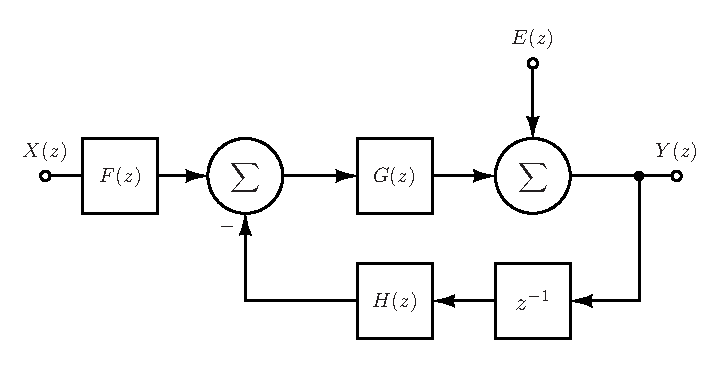
\includegraphics[width=0.8\textwidth]{DTDSM_lin}
	\end{figure}
	%---------------------------------------------------------------------------------
	\vfill	
	%-----------------------
	\begin{equation*}
	\text{STF}(z)=\frac
	{\displaystyle\sum_{k=0}^{N}{\alpha_k z^{-k}}}
	{\displaystyle\sum_{k=0}^{N}{\beta_k  z^{-k}}}
	\qquad
	\text{NTF}(z)=\frac
	{\displaystyle\sum_{k=0}^{N}{\gamma_k z^{-k}}}
	{\displaystyle\sum_{k=0}^{N}{\beta_k  z^{-k}}}	
	\end{equation*}
	%-----------------------
	\vfill \strut	
}

\onslide*{2}{
	\centering
	%---------------------------------------------------------------------------------
	\begin{figure}[h!]
	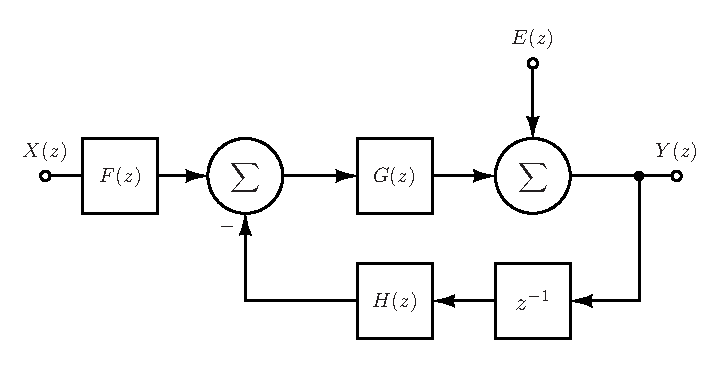
\includegraphics[width=0.8\textwidth]{DTDSM_lin}
	\end{figure}
	%---------------------------------------------------------------------------------
	\vfill
	%-----------------------
	\begin{equation*}
		F(z) = \sum_{k=0}^{N}\alpha_k z^{-k} \qquad 
		G(z) = \sum_{k=0}^{N}\gamma_k z^{k} \qquad
		H(z) = \sum_{k=1}^{N}\left(\beta_k-\gamma_k\right)z^{-k+1}
	\end{equation*}
	%-----------------------
	\vfill \strut
}
\end{slide}


%%% Simulation
\begin{slide}[toc=Simulation,bm=Simulation]{Linear Recursive Difference Equation}

\onslide*{1}{
	\centering
	%-----------------------
	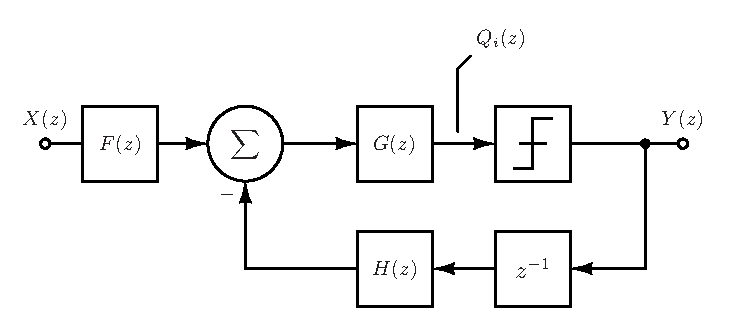
\includegraphics[width=0.8\textwidth]{sim_block_diagram.eps}
	%-----------------------
	\vfill
	%-----------------------
	\begin{equation*}
		Q_i(z) = G(z)\left(F(z)X(z)-z^{-1}H(z)Y(z)\right)
	\end{equation*}
	%-----------------------
	\vfill \strut
}

\onslide*{2}{
	\centering
	%-----------------------
	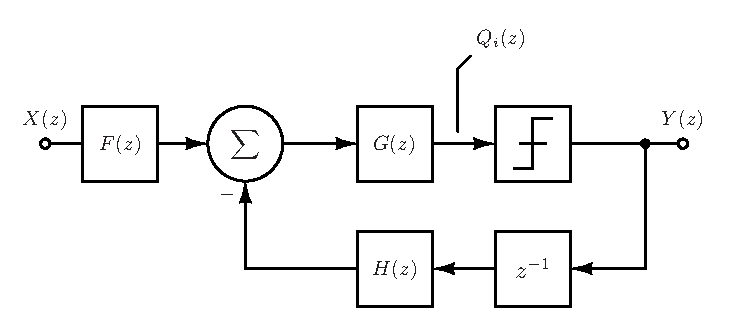
\includegraphics[width=0.8\textwidth]{sim_block_diagram.eps}
	%-----------------------
	\vfill
	\begin{equation*}
		q_i(n)=\sum_{k=0}^{N}\alpha_k
		x(n-k)-\sum_{k=1}^{N}\left(\beta_k-\gamma_k\right)y(n-k)-
		\sum_{k=1}^{N}\gamma_k q_i(n-k)
	\end{equation*}
	%-----------------------
	\begin{equation*}
		y(n)=\mathop\text{sgn}\left[q_i(n)\right]
	\end{equation*}
	%-----------------------
	\vfill \strut
}
\end{slide}

%%% Analysis
\begin{slide}[toc=Analysis,bm=Analysis]{Frequency Domain Analysis}

\onslide*{1}{
	\vfill
	\centering
	Output Decimation Filtering
	%-----------------------
	\includegraphics[width=0.8\textwidth]{decimation_block_diagram}
	%-----------------------
	\vfill

	\begin{itemize}
		\item \DS modulator output, $y(n)$, lowpass filtered by $H_d(z)$
		\vfill
		\item Filtered output, $y_f(n)$, downsampled by a factor of the OSR, $M$
		\vfill
		\item Filtered and downsampled \DS modulator output, $y_d(n)$, is then windowed
			  and analyzed in the frequency domain
	\end{itemize}
	\vfill \strut
}

\onslide*{2}{
	\vfill
	\centering
	Signal-to-Noise Ratio (SNR)
	\vfill
	%-----------------------
	\begin{equation*}\label{eq:SNR_freq}
	\text{SNR}_\text{dB}=10\log\left(\frac{P_s}{P_{n,a}}\right)=10\log\left(\frac
	{
	\displaystyle\sum_{k=K_1}^{K_2}\left\lvert
	Y_w(k)\right\rvert^2
	}
	{
	\displaystyle\sum_{k=0}^{K_1-1}\left\lvert Y_w(k)\right\rvert^2 +
	\sum_{k=K_2+1}^{N/4-1} \left\lvert Y_w(k)\right\rvert^2
	}\right)
	\end{equation*}
	%-----------------------
	\vfill
	\begin{itemize}
		\item $K_1$ and $K_2$ are the FFT bins corresponding to the 
			  leading and trailing edge of the fundamental lobe
		\vfill
		\item SNR is the ratio of the power contained in the fundamental lobe
			  to the noise power in the windowed output spectrum 
	\end{itemize}
	\vfill \strut
}
	
\onslide*{3}{
	\vfill
	\centering
	Dynamic Range (DR)
	\vfill
	%-----------------------
	\begin{equation*}
		\text{DR}_{\text{dB}} =10\log\left(\frac{P_s}{P_{n,p}}\right)=
		10\log\left(\frac{4}{N_pN}\sum_{k=K_1}^{K_2}\lvert Y_w(k)\rvert^2\right)
	\end{equation*}
	%-----------------------
	\begin{equation*}\label{eq:max_noise_floor}
		N_p=\max\langle\lvert Y_{d,e}(k)\rvert\rangle
	\end{equation*}
	%-----------------------
	\vfill
	\begin{itemize}
		\item $K_1$ and $K_2$ are the FFT bins corresponding to the 
			  leading and trailing edge of the fundamental lobe
		\vfill
		\item DR is the ratio of the power contained in the
			  fundamental lobe to an output noise spectrum equal in magnitude
			  to the maximum observed noise component, $N_p$
	\end{itemize}
	\vfill \strut
}
\end{slide}

%%%  DSM OPTIMIZATION RESULTS
\begin{slide}[toc=Results,bm=Results]
{$\Delta\Sigma$ Modulator Optimization Results}

% \onslide*{1}{
% 	%---------------------------------------------------------------------------------
%  	\begin{figure}
%  	\centering 	
% 	\subfigure{
%  	\includegraphics*[width=0.45\textwidth]{2nd_order_mags.eps}
% 	}
%  	\hspace{0.01\textwidth}
%  	\subfigure{
%  	\includegraphics*[width=0.45\textwidth]{2nd_order_output_spectra.eps}
% 	}\\
% 	\subfigure{
%  	\includegraphics*[width=0.45\textwidth]{3rd_order_mags.eps}
% 	}
%  	\hspace{0.01\textwidth}
%  	\subfigure{
%  	\includegraphics*[width=0.45\textwidth]{3rd_order_output_spectra.eps}
% 	}	
% 	\end{figure}
% 	%---------------------------------------------------------------------------------
% }

\onslide*{1}{
	\vfill
	\centering
	5th Order $\Delta\Sigma$ Modulator
	%---------------------------------------------------------------------------------
	\begin{figure}
	\subfigure{
	\includegraphics[width=0.45\textwidth]{5th_order_mags}
	}
	\subfigure{
	\includegraphics[width=0.45\textwidth]{5th_order_output_spectra}
	}
	\end{figure}
	%---------------------------------------------------------------------------------
	\vspace{-7.5mm}
	%---------------------------------------------------------------------------------	
	\begin{table}[htbp]
 		\begin{center}
 		\begin{tabular}{ l c c }\toprule
 		\textbf{Design Method}  & \textbf{SNR$_\text{dB}$} & \textbf{DR$_\text{dB}$}\\	
		\midrule
        DelSig Toolbox   &     83       &     66      \\
        Chebyshev Filter &     81       &     72      \\
        HOG Algorithm    &     87       &     76      \\ \bottomrule
		\end{tabular}
		\end{center}
	\end{table}
	%----------------------------
	\vfill \strut
}

\onslide*{2}{
	\vfill
	\centering
	6th Order $\Delta\Sigma$ Modulator
	%---------------------------------------------------------------------------------
	\begin{figure}
	\subfigure{
	\includegraphics[width=0.45\textwidth]{6th_order_mags}
	}
	\subfigure{
	\includegraphics[width=0.45\textwidth]{6th_order_output_spectra}
	}
	\end{figure}
	%---------------------------------------------------------------------------------
	\vspace{-7.5mm}
	%----------------------------
	\begin{table}[htbp]
 		\begin{center}
 		\begin{tabular}{ l c c }\toprule
 		\textbf{Design Method}  & \textbf{SNR$_\text{dB}$} & \textbf{DR$_\text{dB}$} \\
		\midrule
        DelSig Toolbox   &     88       &     74      \\
        Chebyshev Filter &     87       &     77      \\
        HOG Algorithm    &     91       &     80      \\ \bottomrule
		\end{tabular}
		\end{center}
	\end{table}
	%----------------------------
	\vfill \strut
}
\end{slide}

\begin{slide}[toc=Summary,bm=Summary]
{$\Delta\Sigma$ Modulator Optimization Results}

\onslide*{1}{
	\vfill
	\centering
	OSR: 32\\
	%---------------------------------------------------------------------------------
	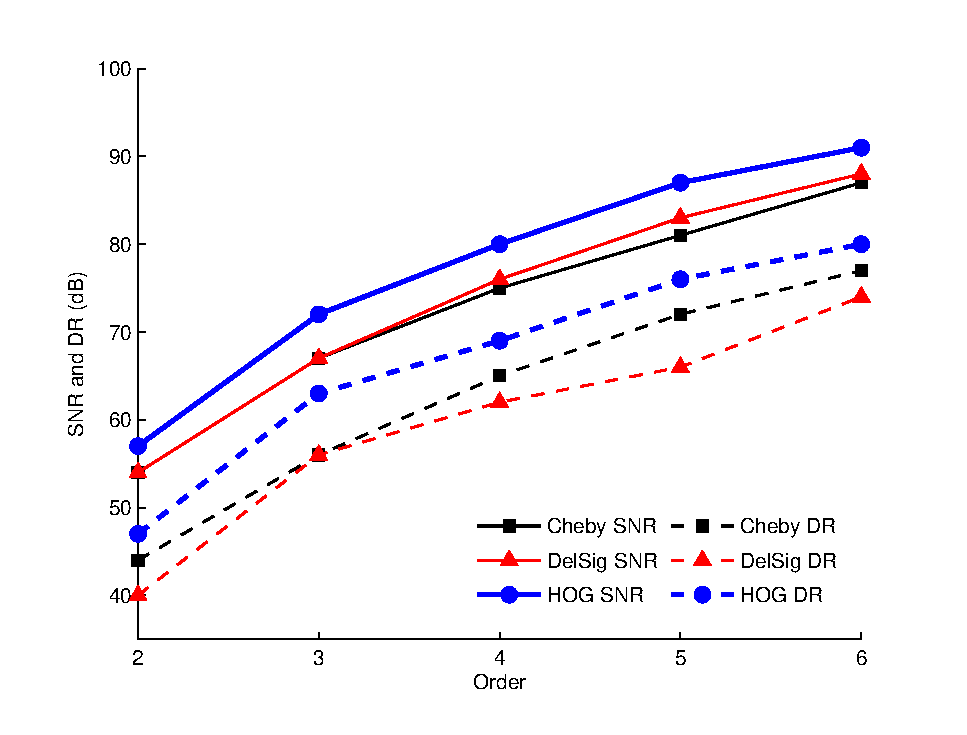
\includegraphics[width=0.9\textwidth]{OSR_32_chart}
	%---------------------------------------------------------------------------------
	\vfill \strut
}

\onslide*{2}{
	\vfill
	\centering
	OSR: 64\\
	%---------------------------------------------------------------------------------
	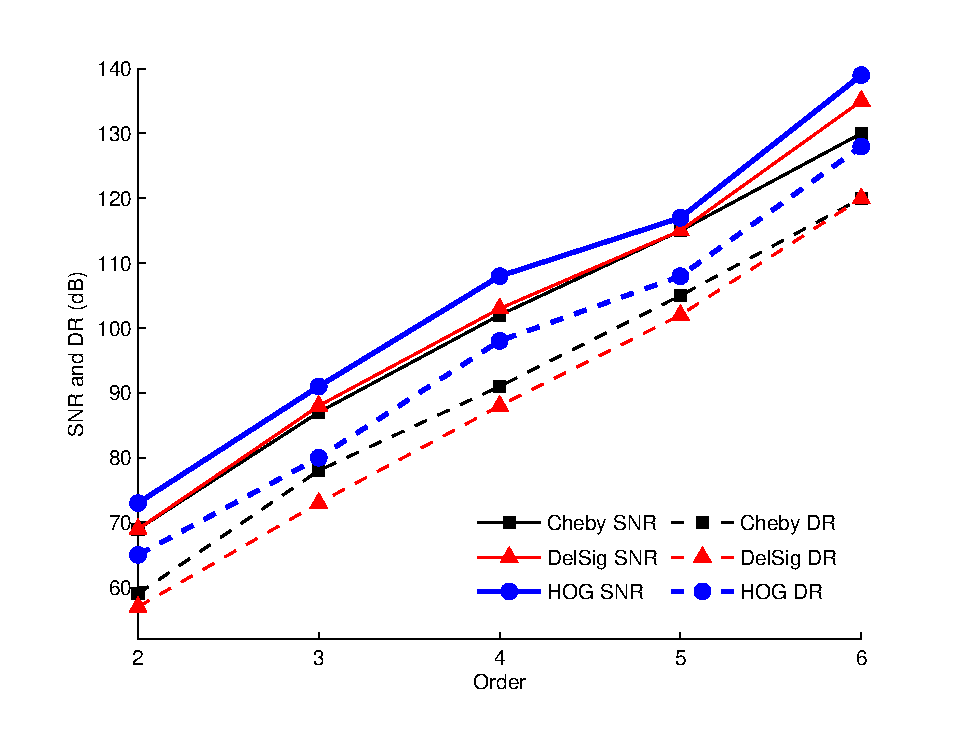
\includegraphics[width=0.9\textwidth]{OSR_64_chart}
	%---------------------------------------------------------------------------------
	\vfill \strut	
}

\onslide*{3}{
	\vfill
	\centering
	OSR: 128\\
	%---------------------------------------------------------------------------------
	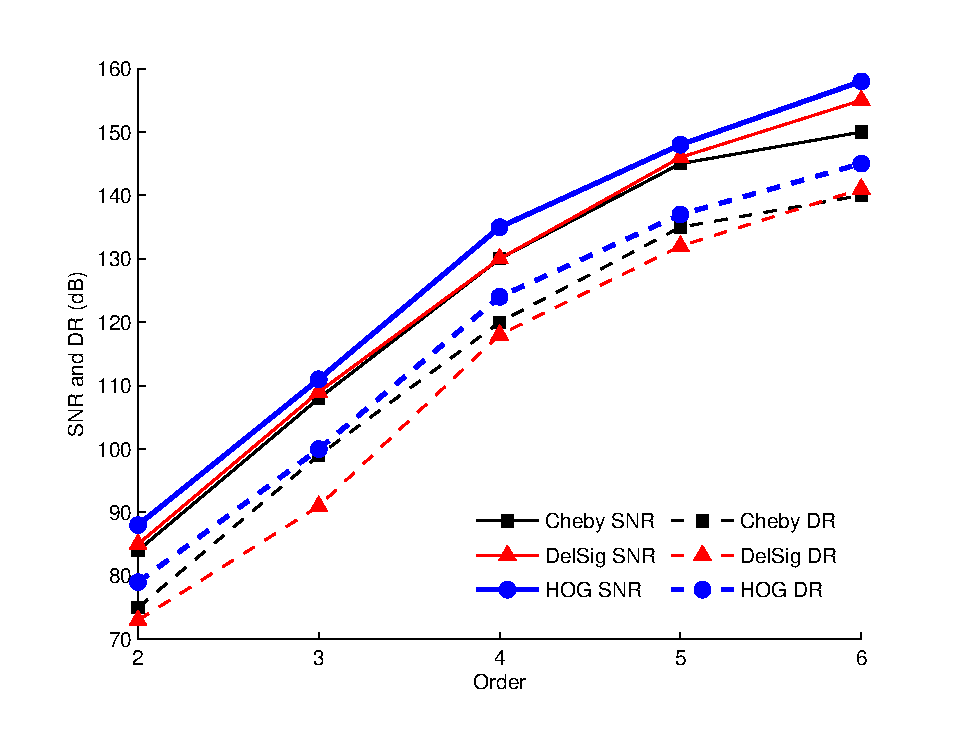
\includegraphics[width=0.9\textwidth]{OSR_128_chart}
	%---------------------------------------------------------------------------------
	\vfill \strut
}
\end{slide}

% 	\vfill
% 	\centering
% 	%---------------------------------------------------------------------------------
%  	\begin{figure}
%  	\centering 	
% 	\subfigure{
%  	\includegraphics*[width=0.31\slidewidth]{OSR_32_chart.eps}
% 	}
% 	\hspace{-0.05\slidewidth}
%  	\subfigure{
%  	\includegraphics*[width=0.31\slidewidth]{OSR_64_chart.eps}
% 	}
% 	\hspace{-0.05\slidewidth}
% 	\subfigure{
%  	\includegraphics*[width=0.31\slidewidth]{OSR_128_chart.eps}
% 	}
% 	\end{figure}
% 	%---------------------------------------------------------------------------------
% 	\vfill \strut
% \end{wideslide}

%%%%%%%%%%%%%%%%%%%%%%%%%%%%%%%%

\section[slide=true]{Conclusions}

%%%%%%%%%%%%%%%%%%%%%%%%%%%%%%%%
%%% HOG CONCLUSIONS
\begin{slide}[toc=HOG Conclusions,bm=HOG Conclusions]{HOG Algorithm Conclusions}
	\vfill
	\begin{itemize}[type=1]
		\item Effectively solves widely accepted benchmark unimodal and multimodal
		problems across a broad range of dimensions \pause
		\vfill
		\item Robust methods inherent to the orthogonal crossover operator increase
		\textit{convergence confidence} by providing repeatable highly-optimized solutions
		which are equivalent to known optimal solutions \pause
		\vfill
		\item Algorithm performance (computational load, mean solution, standard
		deviation, etc) is consistent with similar algorithms 
	\end{itemize}
	\vfill \strut
\end{slide}
%%%%%%%%%%%%%%%%%%%%%%%%%%%%%%%%

%%%%%%%%%%%%%%%%%%%%%%%%%%%%%%%%
%%% OPTIMAL DTDSM CONCLUSIONS
\begin{slide}[toc=DSM Conclusions,bm=DSM Conclusions]
{Optimal \DS Modulator Design Conclusions}
	\vfill
	\begin{itemize}[type=1]
		\item Traditional polynomial based design methods shown to perform as good as
		EDA tool based design techniques for most cases\pause
		\vfill
		\item When compared to both classical polynomial based design techniques and
		contemporary EDA based design techniques, the SNR and DR optimization based design
		was	shown to provide increased DR and SNR thereby increasing the \DS modulator’s
		effective resolution \pause
		\vfill
		\item HOG algorithm based method determines optimal NTFs and STFs with respect to
		SNR and DR
	\end{itemize}
	\vfill \strut
\end{slide}
%%%%%%%%%%%%%%%%%%%%%%%%%%%%%%%%

%%%%%%%%%%%%%%%%%%%%%%%%%%%%%%%%
%%% FUTURE WORK
\begin{slide}[toc=Future Work,bm=Future Work]{Future Work}
	\vfill
	\begin{small}
	\begin{itemize}[type=1]
		\vfill
		\item Modify the HOG algorithm mutation operator to introduce genetic information
			which does not exist in the current population's genotype \pause
		\vfill
		\item Introduce a check-and-repair operator to monitor mutation with respect to 
			the current objective function \pause
		\vfill
		\item Augment the HOG algorithm with a gradient based search method to find the
			optimal value once in the region of the global minimum \pause
		\vfill
		\item Automate stability analysis to \textit{close the loop} for optimal \DS
		modulator design \pause
		\vfill	
		\item Extend the application of the HOG algorithm to include the optimal design of
		continuous-time \DS modulators \pause
		\vfill
		\item Include non-ideal circuit level implementation considerations such as jitter
		tolerance, loop delay, and lossy integration in \DS modulator objective function
		\pause
		\vfill
		\item Implement the updated HOG algorithm as a multiobjective, constrained global
		optimizer to determine Pareto optimal system functions including rigid stability
		criterion
	\end{itemize}
	\end{small}
	\vfill \strut
\end{slide}
%%%%%%%%%%%%%%%%%%%%%%%%%%%%%%%%

%%%%%%%%%%%%%%%%%%%%%%%%%%%%%%%%
%%% QUESTIONS AND DISCUSSION
\begin{slide}[toc=,bm=]{Questions}
\vfill
\begin{figure}[htbp]
 \centering
 \includegraphics*[width=0.7\textwidth,clip,viewport=124 575 471 713]{time.ps}
%  \subfigure{
%  \includegraphics*[width=0.45\textwidth,clip,viewport=124 575 471 713]{edits.ps}
%  }
%  \hspace{0.01\textwidth}
%  \subfigure{
%  \includegraphics*[width=0.45\textwidth,clip,viewport=124 575 471 713]{edits_2.ps}
%  }\\
%  \subfigure{
%  \includegraphics*[width=0.45\textwidth,clip,viewport=124 575 471 713]{variance.ps}
%  }
%  \hspace{0.01\textwidth}
%  \subfigure{
%  \includegraphics*[width=0.45\textwidth,clip,viewport=124 575 471 713]{expectation.ps}
%  }\\
%  \subfigure{
%  \includegraphics*[width=0.45\textwidth,clip,viewport=124 575 471 713]{edits_3.ps}
%  }
%  \hspace{0.01\textwidth}
%  \subfigure{
%  \includegraphics*[width=0.45\textwidth,clip,viewport=124 575 471 713]{.ps}
%  }\\
 \vfill \strut
\end{figure}

\end{slide}
%%%%%%%%%%%%%%%%%%%%%%%%%%%%%%%%
\end{document}
